\documentclass[preview]{standalone}

\usepackage{amsmath}
\usepackage{amssymb}
\usepackage{stellar}
\usepackage{bettelini}

\hypersetup{
    colorlinks=true,
    linkcolor=black,
    urlcolor=blue,
    pdftitle={Stellar},
    pdfpagemode=FullScreen,
}

\begin{document}

\title{Stellar}
\id{storia-neutralita-svizzera}
\genpage

\section{Storia della neutralità svizzera}

\begin{snippet}{neutralita-svizzera-eventi-principali}
    La neutralità svizzera può essere distinta in tre momenti storici importanti:
    \begin{enumerate}
        \item \textbf{Nicolao della Flüe (1417-1487):} uno dei primi sostenitori della neutralità svizzera;
        \item \textbf{Battaglia di Marignano (1515)};
        \item \textbf{Congresso di Vienna (1815)}.
    \end{enumerate}
\end{snippet}

\section{L'influenza esercitata da Nicolao della Flüe}

\plain{Ecco i consigli dati da Nicolao della Flüe nel 1481, secondo una cronaca dell'inizio del XVI
secolo:}

\begin{snippet}{nicolao-flue-parole}
    \begin{center}
        \textit{Non cercate di estendere troppo il territorio della} \\
        \textit{Confederazione, affinché possiate mantenere meglio la pace e} \\
        \textit{l'unità e godere della libertà che vi siete così duramente} \\
        \textit{conquistata. Non immischiatevi troppo in quanto succede} \\
        \textit{all'estero e non alleatevi con le potenze straniere.} \\
        \textit{Cari confederati non accettate doni o denaro, affinché né la} \\
        \textit{gelosia né l'egoismo possano germogliare in voi e avvelenare} \\
        \textit{così i vostri cuori. Mantenete in tutte le relazioni la vostra} \\
        \textit{innata equità, suddividete il bottino a seconda del servizio} \\
        \textit{prestato e assegnate in modo giusto ai cantoni le terre} \\
        \textit{conquistate. Non lasciatevi mai trascinare in guerre ingiuste} \\
        \textit{solo perché intravedete la possibilità di bottino; vivete in pace} \\
        \textit{e in accordo con i vostri vicini. Se dovessero attaccarvi,} \\
        \textit{difendete la vostra patria combattendo da valorosi.} \\
        \textit{Praticate la giustizia nei vostri paesi e amatevi l'un l'altro,} \\
        \textit{come veri alleati cristiani. Non immischiatevi in dispute tra} \\
        \textit{stranieri, mostratevi temibili solo verso coloro che cercano di} \\
        \textit{esprimervi soprattutto evitate le discussioni.}
    \end{center}
\end{snippet}

\section{La battaglia di Marignano}

\plain{Le battaglie espansionistiche della Svizzera continuano fino alla battaglia di Marignano.}

\begin{snippetdefinition}{battaglia-marignano-definizione}{Battaglia di Marignano}
    La \textit{battaglia di Marignano} fu uno scontro armato avvenuto tra il 13 e 14
    settembre 1515 a Melegnano e San Giuliano Milanese,
    16 km a sud est di Milano per il controllo del Ducato di Milano. 
\end{snippetdefinition}

\begin{snippet}{35b6149a-198d-42dc-9bff-e05d1b93f6ed}
    La battaglia vide la vittoria dell'alleanza franco-veneta
    e - verso la fine della battaglia - dalle forze della Repubblica di Venezia.
    Sul fronte opposto erano schierati gli svizzeri, che dal 1512 avevano il controllo
    effettivo del Ducato di Milano.
\end{snippet}

\begin{snippet}{marignano-ritirata-illustration}
    \begin{center}
    \begin{figure}[h]
        \centering
        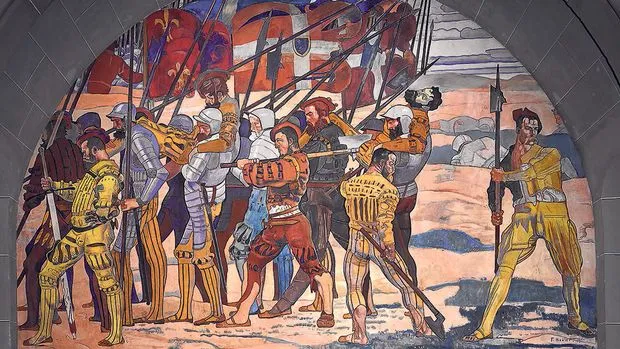
\includegraphics[width=0.9\textwidth]{./resources/marignano_ritirata.png}
        \caption{Ritirata degli svizzeri}
    \end{figure}
    \end{center}
\end{snippet}

\begin{snippet}{3726b9be-ae7f-4b5c-ac97-01c37007be0c}
    Dal 1515 la Svizzera assume un comportamento tendenzialmente \quotes{neutrale}.
    La disfatta di Marignano ha spezzato lo slancio espansionistico dei confederati.
    Nello stesso periodo i cantoni svizzeri hanno sottoscritto una serie di
    alleanze e di trattati che li legano alle potenze vicine
    (Francia, Austria, Savoia e Spagna).
    
    Le \textbf{divisioni religiose} impediscono agli svizzeri di condurre una politica estera comune. I due
    gruppi confessionali vivono in uno stato di equilibrio assai precario. Ogni alleanza di uno di
    questi blocchi con lo straniero provocherebbe una reazione dell'altro e potrebbe scatenare una
    \textbf{guerra civile}.
    
    Nel XVII secolo i cantoni svizzeri praticano una neutralità ancora imperfetta, che non è
    riconosciuta dagli altri Stati. Interi reggimenti di soldati e di mercenari svizzeri combattono in
    tutta l'Europa; alcuni cantoni concedono il diritto di transito a truppe straniere. Ma, dalla metà
    del XVII secolo, si delinea una chiara evoluzione verso il rafforzamento della neutralità. Nel
    1647, con il defensionale di Wil, si fa strada l'idea di una \textbf{neutralità armata}. Dopo il 1648 i
    cantoni decidono di non più concedere alcun diritto di transito sui valichi svizzeri alle truppe
    straniere. Nel 1674 la Dieta federale dichiara che il Corpo elvetico si comporterà da Stato
    neutrale e che non parteciperà in alcun modo alla guerra che coinvolge numerosi Stati europei.
    
    Per tutto il XVIII secolo gli svizzeri si dimostrano prudenti e rimangono lontani dai conflitti
    europei. Il periodo rivoluzionario francese (1789- 1799) metterà i cantoni di fronte a un grave
    pericolo. Nel 1798 le truppe repubblicane francesi, accolte qua e là con entusiasmo, penetrano
    in Svizzera e la occupano. Da quel momento la neutralità Svizzera cessa di esistere; nel 1798 la
    Repubblica elvetica deve sottoscrivere un'\textbf{alleanza offensiva} e difensiva con la Francia; oltre
    a ciò gli svizzeri assicurano alle autorità francesi un contingente di 18.000 uomini. Con
    l'avvento di Napoleone la situazione non evolve affatto in favore dell'indipendenza della
    Svizzera. Il primo console riappacifica il paese con l'Atto di Mediazione (1803), ma continua a
    dettare la politica estera dei cantoni. Ottiene il diritto di assoldare quattro reggimenti svizzeri
    per un totale di 16.000 uomini. Obbliga le autorità cantonali a mettere in atto il blocco
    economico contro i prodotti inglesi. Tuttavia la stella dell'imperatore francese tramonta con la
    grave sconfitta subita in Russia. Dopo la disfatta di Lipsia gli eserciti della coalizione
    antifrancese si avvicinano al Reno.
\end{snippet}

\section{Congresso di Vienna}

% Charkes Pichet de Rochemont (1755-1824) riesce ad otten...

\section{Affari dei colonnelli}

\begin{snippetdefinition}{affare-dei-colonnelli-definizione}{Affare dei colonnelli}
    Dall'inizio della prima Guerra mondiale,
    in virtù di un accordo tra lo Stato maggiore generale sviz.
    e quelli degli Imperi centrali, i colonnelli Friedrich Moritz von Wattenwyl e Karl Egli,
    membri dello Stato maggiore generale, trasmisero agli addetti militari ted. e austro-ungarici
    il bollettino giornaliero del comando supremo sviz. e diversi dispacci diplomatici decifrati
    dai servizi sviz.; si trattava di informazioni il cui valore e grado di confidenzialità
    erano diseguali.
\end{snippetdefinition}

\section{Affare Grimm-Hoffmann}

\begin{snippetdefinition}{affare-grimm-hoffmann-definizione}{Affare Grimm-Hoffmann}
    Nella primavera del 1917,
    l'\textit{affare Grimm-Hoffmann} provocò una grave crisi,
    anche se di breve durata. Nel maggio di quell'anno, 
    Robert Grimm, Consigliere nazionale, membro dirigente della 
    Commissione socialista intern., si recò a Stoccolma, poi 
    a Pietrogrado (oggi San Pietroburgo) per preparare - così ufficialmente - 
    il ritorno dei rifugiati russi nel loro Paese. 
    Ufficiosamente, e con il sostegno del Consigliere fed. Arthur Hoffmann, 
    capo del Dip. politico, che agiva senza il consenso dei suoi colleghi, 
    Grimm tentò di favorire una pace separata tra la Germania e la Russia. 
    A Pietrogrado tenne alcune conferenze e partecipò a una riunione della Commissione
    socialista intern. In occasione di tali incontri entrò in contatto con numerosi
    ministri e personalità vicine al governo e propose loro i suoi buoni uffici.
    Il 26 maggio telegrafò a Hoffmann, comunicandogli che una pace separata
    sembrava possibile e chiedendo precisazioni in merito agli scopi dei belligeranti.
\end{snippetdefinition}

\begin{snippet}{b31b6929-b78d-432d-be69-b1e2333d6998}
    Questi due affari mostrano come la politica estera della svizzera possa essere a volte controversa circa
    la propria neutralità.
    Quando la neutralità viene messa in discussione, si rischia la disgregazione della svizzera.
\end{snippet}

\section{Svizzera come membro della Società delle Nazioni}

\begin{snippet}{bccc0d7a-2195-4650-9c69-d757951be6b7}
    Giuseppe Motta, a capo degli affari esteri, è favorevole all'entrata della Svizzera
    All'interno della Società delle Nazioni.
    
    I membri della Società delle Nazioni hanno il diritto di attendersi che il popolo
    svizzero non voglia astenersi se si tratta di difendere gli alti principi della Società. In
    questo senso il Consiglio della Società ha preso conoscenza delle dichiarazioni fatte
    dal governo svizzero nel suo messaggio all'assemblea federale del 4 agosto 1919 e
    nel suo memorandum del 13 gennaio 1920, dichiarazioni che sono state confermate
    dai delegati svizzeri alla riunione del Consiglio e secondo le quali la Svizzera
    riconosce e proclama i doveri di solidarietà che le risultano dal fatto che sarà membro
    della Società delle Nazioni, compreso il dovere di partecipare alle misure
    commerciali e finanziarie chieste dalla società delle nazioni contro uno Stato in
    rottura del Patto, ed è pronta a tutti i sacrifici per difendere essa stessa il suo
    territorio in qualsiasi circostanza, anche durante un'azione intrapresa dalla Società
    Nazioni, ma che non sarà obbligata a partecipare ad un'azione militare o ammettere
    il passaggio di truppe straniere o la preparazione di imprese militari sul suo
    territorio.
    
    Accettando queste dichiarazioni il Consiglio riconosce che la neutralità perpetua
    della Svizzera e la garanzia dell'inviolabilità del suo territorio così come sono
    acquisite dal diritto delle genti, in particolare dai trattati e l'Atto di 1815, sono
    giustificate dagli interessi della pace generale e, di conseguenza, sono compatibili con
    il Patto.
    
    La Svizzera entra a far parte della Società delle Nazioni con una neutralità differenziata
    (in contraso alla neutralità integrale).
    Questa neutralità è uno strumento flessibile in quanto può essere rielaborata in base
    agli interessi nazionali. La Svizzera usa la neutralità come un mezzo
    per rimanere coesa piuttosto che come uno scopo.
    
    Nella Svizzera francese il consenso era quello di entrare a fare parte della società
    della nazione, mentre in quella tedesca l'opposto.
    Questa spaccatura culturale è dovuto dalla simpatia verso Francia e Germania
    rispettivamente.
    
    La situazione internazionale europea e mondiale sta mutando (accordi di Pace,
    ridisegnano i confini etc.) e chi è favorevole all'entrata della
    Svizzera nella società della Nazioni usa proprio questa argomento come motivazione;
    nel particolare periodo storico dove tutto muta è auspicabile che la Svizzera
    ne entri a far parte. Inoltre, essendo la Svizzera un esponente della pace
    non può sottrarsi completamente dalle interazioni con la società delle Nazioni.
    % guglielmo tell come simbolo di salvezza contro l'invasione straniera.
    Il timore è quello della perdita di indipendenza nei rapporti con l'estero
    e di essere coinvolti in conflitti se si fosse abbandonata la neutralità integrale.
    
    % testo di Motta
    Secondo Motta, nel 1937 la società delle Nazioni non è la stessa organizzazione
    rivolta alla pace degli anni '20, e sarebbe quindi forse il caso di fare un passo indietro.
    La società delle Nazioni non ha nemmeno tanta forza. Infatti, l'Italia non rispetta
    le proprie sanzioni. 
\end{snippet}

\end{document}